\section{Modes of Parallel Execution}

\begin{figure}[t]
  \centering
  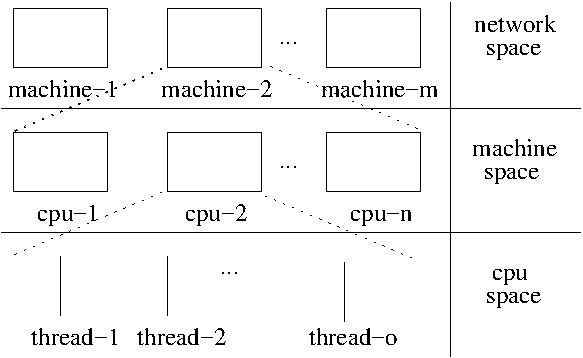
\includegraphics[width=0.4\textwidth]{figs/parallel-levels.pdf}
  \caption{\label{fig:levels}Levels of parallelism.}
\end{figure}

\Fix{write a short paragraph to explain this figure.  explain why
  user/forked thread that run in a (logical) cpu can help speedup?
  assuming i/o?}

\Fix{...explain different modes of parallel execution offered by build
  system and or testing framework...(don't use much more than a column
  of space)}

Modern build systems provides a means to reveal test flakiness.  The
typical approach is to iteratively execute the test suite multiple
times and to mark tests that produce both pass and failing outputs.
More precisely, the developer determines a bound N for the number of
re-executions of the test suite.  Only tests that fail in one given
iteration (consequently, failed in all previous iterations) are
scheduled for re-execution in the next iteration.  At the end of the
process, a test is considered passing if it passes in the first
iteration, a test is considered failing if it fails in all iterations,
and it is considered flaky if it fails in all iterations but the last
it executed.  The process terminates when all tests eventually pass or
when bound N is reached.  Note that every iteration runs a subset of
the test from the previous iteration so execution cost is lower
compared to executing the suite N times.  To note that ITE is
supported by the popular maven surefire
plugin~\cite{maven-surefire-plugin}.\Fix{mention which
  flag/parameter...} ITE provides a means to acknowledge the presence
of test flakiness, including \pef{}s.  Ideally, one would like to
eliminate \pef{}s and avoid the need for ITE.
